\documentclass{article}

\usepackage{tikz}
\usetikzlibrary{calc,fit,shapes,arrows}

\usepackage{listings}

\newcommand{\informed}[0]{{\sc informed}}

\title{Stopwatch architecture design using \informed}


\lstdefinelanguage{SPARK}{
  language = [95]Ada,
  morekeywords = {pre,post,assert,assume,check,derives,hide,global,inherit,from,own,initializes,main_program},
  comment=[l][commentstyle]{--\ },
  texcl=true,
  showstringspaces=false
}

\lstdefinestyle{tinystyle}
   {basicstyle=\footnotesize\tt,
    keywordstyle=\color{blue},
    commentstyle=\rmfamily\it\color{gray},
    captionpos=b,
    caption={},label={},
    numbers=none,
    escapeinside={(*}{*)}}

\lstset{language=SPARK}
\lstset{style=tinystyle}


\tikzstyle{main}=[regular polygon,
                  regular polygon sides=3,
                  draw,
                  minimum width=1cm,
                  inner sep=0.05cm,
                  text badly centered,
                  font=\scriptsize]
\tikzstyle{var}=[draw,
                 text badly centered,
                 text width=1cm,
                 font=\scriptsize]
\tikzstyle{type}=[rectangle,
                  draw,
                  rounded corners,
                  minimum width=1cm,
                  minimum height=0.5cm,
                  text badly centered,
                  font=\scriptsize]
\tikzstyle{boundary}=[single arrow,
                      draw,
                      shape border rotate=270,
                      single arrow head extend=0.0cm,
                      minimum height=0.75cm,
                      minimum width=0.75cm,
                      single arrow tip angle=120,
                      text badly centered,
                      text width=0.75cm,
                      font=\scriptsize]
\tikzstyle{utility}=[trapezium,
                     trapezium left angle=100,
                     trapezium right angle=100,
                     draw,
                     minimum width=.75cm,
                     minimum height=0.5cm,
                     inner sep=0.01cm,
                     minimum height=0.5cm,
                     text badly centered,
                     font=\scriptsize]

\tikzstyle{strong}=[-triangle 90]
\tikzstyle{weak}=[-open triangle 90]



\begin{document}

\section{Diagram}

\begin{figure}[h]
  \begin{center}
    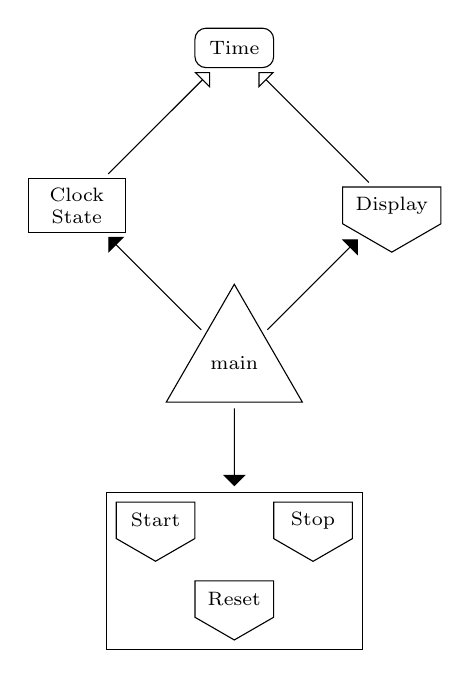
\begin{tikzpicture}[x=2cm,y=2cm,shorten >=2pt, shorten <=2pt]
      \node[main] (main) at (0, 0) {main};

      \node[var] (clock_state)                  at (-1, 1) {Clock\\State};
      \node[boundary, text width=1cm] (display) at ( 1, 1) {Display};
      \node[type]     (time)                    at ( 0, 2) {Time};

      \node[boundary] (start)       at (-0.5, -1) {Start};
      \node[boundary] (stop)        at ( 0.5, -1) {Stop};
      \node[boundary] (reset)       at ( 0, -1.5) {Reset};

      \node[draw, fit=(start) (stop) (reset)] (buttons) {};

      \draw[->,strong] (main) -- (clock_state);
      \draw[->,strong] (main) -- (display);
      \draw[->,weak] (clock_state) -- (time);
      \draw[->,weak] (display) -- (time);
      \draw[->,strong] (main) -- (buttons);
    \end{tikzpicture}
  \end{center}
  \caption{\informed\ diagram of our Stopwatch}
\end{figure}

\pagebreak
\section{\informed\ package structure}

\subsection{Time}
\lstinputlisting{spark/time.ads}

\subsection{Clock State}
\lstinputlisting{spark/clock.ads}

\subsection{Display}
\lstinputlisting{spark/display.ads}

\subsection{Controls}
\lstinputlisting{spark/controls.ads}

\subsection{Main}
\lstinputlisting{spark/main.adb}

\end{document}
